\subsection{Fixed-image comparisons and reference effects}
Table~\ref{tab:cross} holds the accepted image set fixed within each column.
\begin{table}[t]
\caption{Cross-evaluation at 80\% coverage: mean complete-vote disagreement (\%) across seeds. Rows hold predictions fixed; columns hold accepted images fixed}\label{tab:cross}
\centering\begin{tabular}{llrr}\toprule
State & Predictor & Uniform set & Soft set\\\midrule
selected & Uniform & 24.062 & 24.037\\
selected & Soft & 24.148 & 23.684\\
epoch12 & Uniform & 23.949 & 23.846\\
epoch12 & Soft & 24.037 & 23.632\\
\bottomrule\end{tabular}

\end{table}

On Uniform-selected images, Soft minus Uniform is +0.085 pp; on Soft-selected images it is -0.352 pp. Within a column, annotations and the floor are identical, so the risk difference is also a category-choice excess difference on that image set. Holding the Uniform predictor fixed, changing from its own set to the Soft set changes risk by -0.025 pp; for the Soft predictor the corresponding change is -0.463 pp. Thus, the own-set contrast is not a consistent category-choice improvement on a fixed image set. Predictor and selector interact; these cross-evaluations are not a unique causal decomposition. The mean Jaccard overlap is 0.8408; individual intersections and overlap fractions are released.
\begin{table}[t]
\caption{Selected-model weighted F1 with population and reference separated; means across three seeds}\label{tab:samef1}
\centering\begin{tabular}{lrrr}\toprule
Targets & Original/all & Original/subset & Crowd/subset\\\midrule
Hard & 0.5658 & 0.6580 & 0.8965\\
Tie-hard & 0.5599 & 0.6572 & 0.9032\\
Uniform & 0.5683 & 0.6642 & 0.9205\\
Tie-Uniform & 0.5662 & 0.6619 & 0.9195\\
Soft & 0.5722 & 0.6685 & 0.9270\\
\bottomrule\end{tabular}
All: 3,275 images; subset: the same 2,484 supported-majority images in the last two columns. No retraining or relabeling is performed.
\end{table}

In Table~\ref{tab:samef1}, the last two columns hold the image population fixed while changing the categorical reference. The first two hold the original-label reference fixed while changing the population. Their differences therefore disentangle two sources of the superficially large original-versus-crowd F1 contrast. The reference confusion matrix is supplied in the supplement; neither reference is treated as emotional truth.
\begin{figure}[t]\centering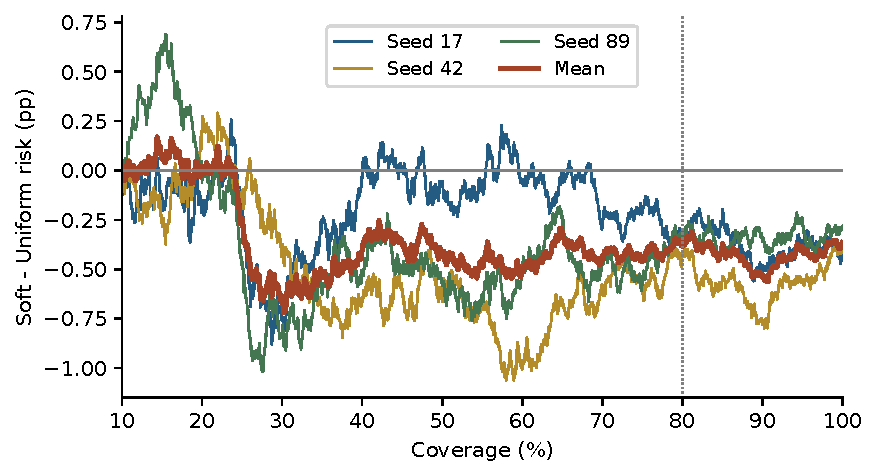
\includegraphics[width=\linewidth]{evidence_revision/figures/RiskDifference.pdf}
\caption{Soft-minus-Uniform complete-vote disagreement versus common coverage. Thin curves are paired seeds; the thick curve is their mean. Curves use each model's own ranking, not identical image sets. The vertical marker identifies the primary 80\% endpoint; this descriptive curve has no simultaneous uncertainty band}\label{fig:difference}\end{figure}
\subsection{Tie-preserving dominant-confidence control}
Table~\ref{tab:tieuniform} reports both checkpoint states for the new secondary comparison.
\begin{table}[t]
\caption{Secondary matched Tie-Uniform comparison at 80\% coverage. Risks are percentages; differences and conditional 95\% intervals are percentage points}\label{tab:tieuniform}
\centering\begin{tabular}{lrrrr}\toprule
State & Tie-Uniform & Soft & Difference & Interval\\\midrule
selected & 24.272 & 23.684 & -0.588 & [-0.830, -0.281]\\
epoch12 & 23.939 & 23.632 & -0.307 & [-0.585, -0.024]\\
\bottomrule\end{tabular}

\end{table}

Selected: paired Soft-minus-Tie-Uniform differences are -0.378, -0.584, -0.802 pp for seeds 17, 42, and 89. The conditional interval lies below zero. Epoch12: paired Soft-minus-Tie-Uniform differences are -0.435, -0.221, -0.263 pp for seeds 17, 42, and 89. The conditional interval lies below zero. This secondary comparison removes canonical tie asymmetry from Uniform but still changes target entropy and class marginals relative to Soft. It cannot isolate a unique minority-category identity mechanism.
\begin{table}[t]
\caption{Selected epochs under the common distribution-distance criterion}\label{tab:epochs}
\centering\begin{tabular}{lrrr}\toprule
Targets & Seed 17 & Seed 42 & Seed 89\\\midrule
Hard & 3 & 2 & 5\\
Tie-hard & 4 & 4 & 5\\
Uniform & 9 & 6 & 10\\
Tie-Uniform & 12 & 8 & 7\\
Soft & 9 & 10 & 10\\
\bottomrule\end{tabular}

\end{table}

Training-loss and selection-distance trajectories are supplied for every run in the supplement. Loss scales differ by target construction and are not directly comparable evidence of better fitting.
\subsection{Retention of unsupported categories}
Table~\ref{tab:retention} retains individual seed counts rather than only a mean ordering.
\begin{table}[t]
\caption{Accepted image counts at global 80\% coverage, seeds 17, 42, 89 in that order. Population sizes: full 1,732; partial 1,527; zero 16}\label{tab:retention}
\centering\begin{tabular}{lrrr}\toprule
Targets & Full mass & Partial mass & Zero mass\\\midrule
Hard & 1499, 1501, 1492 & 1115, 1112, 1122 & 6, 7, 6\\
Tie-hard & 1519, 1494, 1508 & 1092, 1119, 1106 & 9, 7, 6\\
Uniform & 1515, 1527, 1527 & 1098, 1087, 1085 & 7, 6, 8\\
Tie-Uniform & 1529, 1522, 1520 & 1084, 1090, 1095 & 7, 8, 5\\
Soft & 1527, 1527, 1533 & 1081, 1083, 1076 & 12, 10, 11\\
\bottomrule\end{tabular}
Each seed retains 2,620 images in total. Zero-mass images have disagreement one under every supported prediction.
\end{table}

Soft retains 11.00 of the 16 zero-supported-mass images on average, versus 7.00 for Uniform and 6.67 for Tie-Uniform. Better aggregate risk therefore does not imply better rejection of wholly unsupported annotations. These small counts are descriptive, not an estimated deployment failure rate. Contempt, unknown and not-a-face vote-mass breakdowns are supplied separately rather than interpreted as one semantic category.
Before confidence selection, calibration vote mass is 1.797\% contempt, 3.666\% unknown, and 0.262\% not-a-face. Before confidence selection, test vote mass is 1.554\% contempt, 5.667\% unknown, and 0.656\% not-a-face. These are vote fractions, not counts of images; the accepted-set breakdown in the supplement conditions on each ranking.
